\section{Interactions of pedestrians and automated vehicles}
\label{chap1b:sec2}
Extensive presence of automated vehicles in urban areas is going to be one of the major changes in near future. In urban areas altered fundamentally by the presence of AVs, studying pedestrians' crossing behaviour is of paramount importance, for the safety of most vulnerable users, optimal roadway layout changes, geometric design updates, and traffic flow optimization. The necessity for new approaches in studying pedestrian and vehicle interactions with an emphasis on investigating mid-block unsignalized crossings raises as AVs, as the rule-obeying agents of future urban space, are expected to always yield to crossing pedestrians~\cite{millard2018pedestrians}. In \cref{fig:frameworkcross}, dynamics of a mid-block unsignalized crossing of a pedestrian is depicted. On the pedestrian's side, waiting on the side walk for a safe gap to initiate a cross, and following a trajectory and its corresponding speed and acceleration to reach the other side of the street are the two behaviours of a crossing pedestrian. Reactions of the vehicle based on the observation of the environment and prediction of pedestrian's behaviours form the vehicle side of the dynamics. The next two sections explore the two parts of the pedestrian side of the these interactions: wait time and trajectory.
\begin{figure}
    \centering
    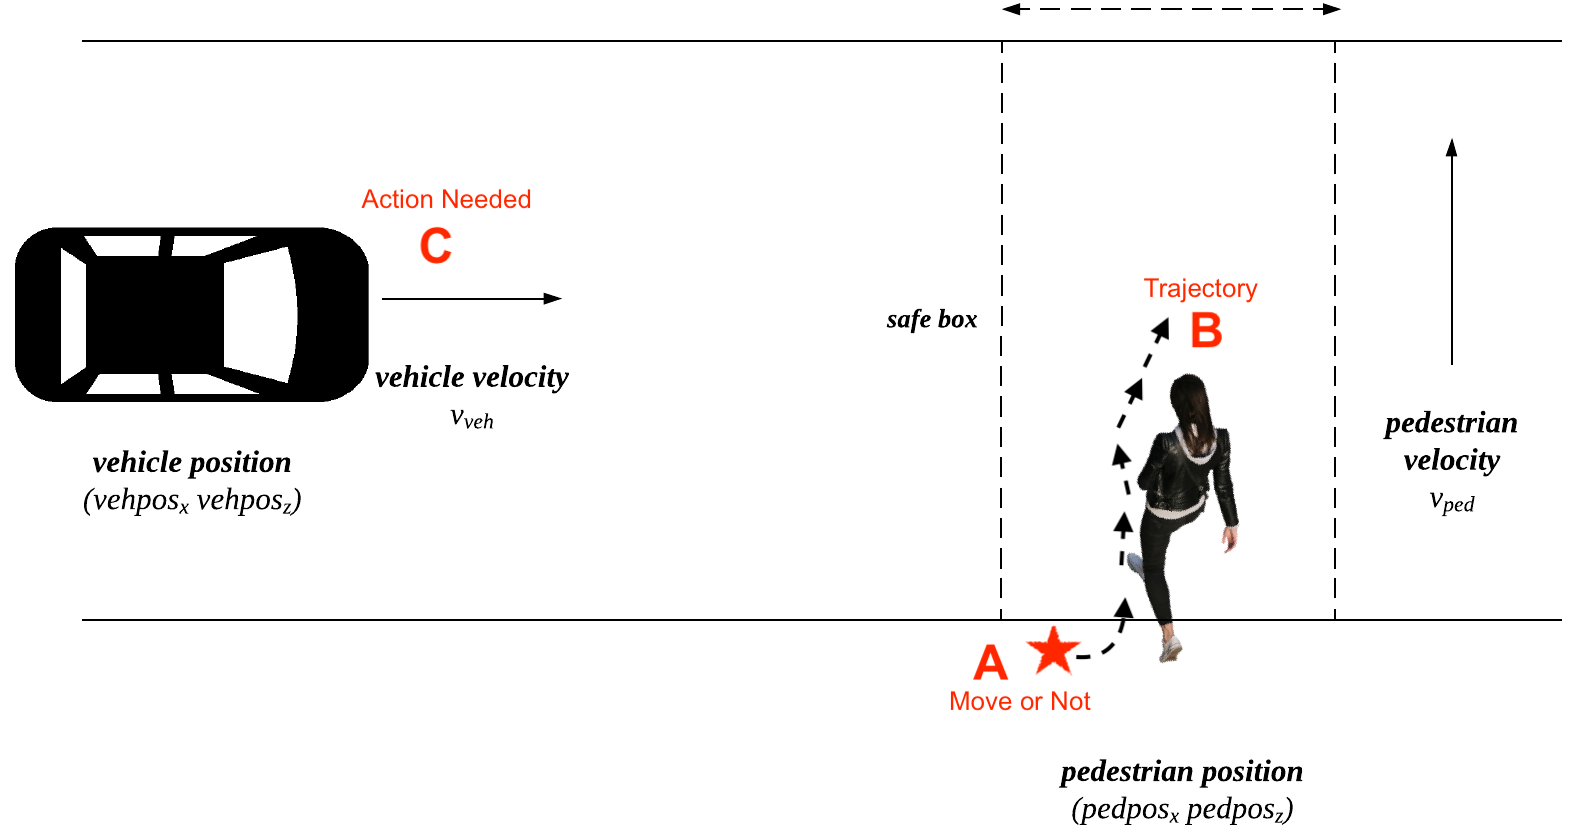
\includegraphics[scale=0.2]{chapter_1b/figures/ped5.png}
    \caption{Vehicles and pedestrians interactions in mid-block crossings}
    \label{fig:frameworkcross}
\end{figure}

\subsection{Pedestrian wait time analysis}
Most studies in pedestrian wait time at unsignalized intersections and mid-block crossings focus on the concept of accepted gap time. Wilson and Grayson~\cite{wilson1980age} analyzed pedestrians' accepting gaps of less than 2 seconds, which is considered to be very short, at a crossing with two-way traffic flow, for different age groups. Results showed that 3.4\% of males and 2\% of females accept these gaps when crossing against nearside traffic. Acceptance rate of such gaps when crossing against far side traffic was higher at 6.2 and 4.8\%, respectively.
On a similar study considering medians, Das~\textit{et al.}~\cite{das2005walk} found that pedestrians waiting on medians accept shorter gaps more easily, compared to those waiting on the curb sides.  According to this study, pedestrians behave more cautiously confronting bigger vehicles. However, the effect of waiting times and number of crossing attempts are not taken into account in this study. In an older study, DiPietro and King~\cite{dipietro1970pedestrian} considered waiting time in their gap time analysis and concluded that by increasing waiting time on the curb, the accepted gaps increases as well. In other words, pedestrians who wait longer before crossing require longer gaps between cars to cross the road. Considering gender of the pedestrians, the results revealed that men were willing to cross using shorter gaps in comparison to women. Moreover this study suggested that, despite having slower pace, pedestrians in group accept shorter gaps than individuals. This finding can be traced back to a couple of reasons, such as the effect of peer pressure to cross, lack of attention, or perception of safety in numbers. Oxley~\textit{et al.}~\cite{oxley2005crossing} focused on the effect of age on the ability to choose safe gap time. By developing a logistic regression model, gap selection was analyzed in their study with respect to walking time, age group, time (or distance) gap and vehicle speed. According to their results, the primary contributing factor in deciding to cross, which can be interpreted as waiting time, appeared to be the distance to upcoming vehicle and time of arrival. Moreover, elderly participants appeared to select more unsafe gap times, given that their walking speeds were slower. In a relatively more recent work, Kadali~\textit{et al.} used Artificial Neural Networks (ANN) to estimate pedestrians' gap acceptance at mid-block unmarked crossings and compared its performance to multiple regression models. Their results showed that ANN has a better prediction performance, being able to consider the effects of higher number of variables. However, the authors mentioned the strength of regression models in such cases due to their ability to reflect the significance of contributing variable. A few researchers have employed game theory models to study pedestrian-vehicle interactions for mid-block unmarked crossings. Sun~\textit{et al.}~\cite{sun2003modeling} for instance, developed a framework for pedestrian-vehicle interaction based on pedestrians’ gap acceptance and motorists yield behaviour. With respect to pedestrians gap acceptance, three types of models were explored: a deterministic model considering gap size, a probabilistic model assuming a certain distribution for gap acceptance as a random variable, and a binary logit model considering age, gender, waiting time, gap size, and number of pedestrians waiting on the curb. Finally, pedestrian and vehicle interactions were modelled as a two-player non-zero-sum non-cooperative game. 

Some studies have tried to model wait time directly, and not through the lens of accepted gap times. In one of the earliest studies of pedestrian crossings at unsignalized crosswalks, Hamed~\cite{hamed2001analysis} used data collected from observations in the city of Amman, Jordan, to investigate the pedestrian waiting time at mid-block locations on divided and undivided roads. A Cox Proportional Hazards (CPH) model was developed to model pedestrian waiting time on the sidewalks. The results suggested that having accident experience, car ownership, number of people on the crosswalk, age, gender, type of trip and vehicle gap time are important factors in determining wait time before crossing. It is interesting to note that the parameters related to traffic were not found to be statistically significant. In another study, Tiwari~\textit{et al.}~\cite{tiwari2007survival}, observed that the average waiting time for females is 27\% more than for males at signalized intersections. In a similar work, Wang~\textit{et al.}~\cite{wang2011individual} developed a parametric survival analysis and found that personal characteristics affect crossing behaviour. In their sample group of study, young men on their way to school were more likely to terminate their waiting time in shorter time. They also indicated that crossing behaviour is highly influenced by safety awareness and conformity behaviour. In another study on modeling pedestrians' waiting time at signalized intersections, Li~\cite{li2013model} applied a statistical modeling approach and proposed a U shaped distribution for pedestrian waiting time at signalized intersections. By developing the model for different age cohorts, it was concluded that the waiting time increases with age.

In a dominant part of the relevant research, survival analysis has proved to be a powerful tool in investigating and understanding the time before an event occurs and the contributing factors in determining that time. In survival analysis, the aim is to estimate time until an event occurs. A collection of statistical modeling methods can be designed for this purpose. The most common methods for survival analysis are the Kaplan-Meier model~\cite{kaplan1958nonparametric} and Cox Proportional Hazard~\cite{cox1972regression} model. The Kaplan-Meier model is a non-parametric model for estimating the survival function in homogeneous groups. This model is very easy to implement, but is unable to account for individuals. To take into account feature vectors and compute survival functions for individuals, Cox Proportional Hazards model is usually the solution. Cox Proportional Hazards model is a semi-parametric model that assumes time component and feature component of hazards function to be proportional. The strength of survival analysis methods in modeling duration times in various fields, particularly in medical research, makes them a suitable approach to analyze wait time.

\subsubsection{Machine learning models for wait time analysis}
Despite being the common method of survival analysis for years, the assumptions made in Cox Proportional Hazards are not always true and have limitations:
\begin{itemize}
    \item It assume a linear combination of features within the hazards function.
    \item It assumes a constant hazards function over time.
\end{itemize}
To address these issues, Chun-Nam Yu~\textit{et al.}~\cite{yu2011learning} introduced the Multi-Task Logistic Regression model. The proposed model in their study can be interpreted as having different time intervals with different logistic regression models estimating the probability of occurrence of an event in that specific time interval. Although Multi-Task Logistic Regression models address some of the problems of the previous methods, they still remain linear, thus they cannot capture the nonlinear complexities within the data. Several researchers, particularly in the field of medical sciences, have tried to address this issue by implementing a deep learning approaches ~\cite{faraggi1995neural,katzman2016deep,luck2017deep}. Faraggi and Simon~ \cite{faraggi1995neural} first incorporated a feed-forward neural network as a shift to nonlinear proportional hazards models. In their model, they replaced the linear combination of features with the output of a neural network with one output node. However, research followed by suggested that their network did not perform better that linear Cox Proportional Hazards models~\cite{mariani1997prognostic}. As the mentioned work were done prior to the outburst of modern deep learning algorithms, Katzman~\textit{et al.}~\cite{katzman2016deep} decided to test the performance of more recent deep networks on survival models. They added fully connected and dropout layers and outperformed the performance of previous linear Cox Proportional Hazards models.

\subsection{Pedestrian movement modeling}
Modeling pedestrian movements is of vital importance in designing sidewalks and venues, planning events, evacuation scenarios, or in from the perspective of an automated vehicle, to predict the next locations of pedestrians. However, due to the inherent irregularity in pedestrians movements~ \cite{bierlaire2003behavioral}, modeling pedestrians may seem more difficult than that of vehicles. In addition, data collection seems to be a bigger problem when it comes to pedestrians, due to the chaotic movements, larger datasets required and pedestrians not necessarily following predefined routes~\cite{danalet2014bayesian}. To capture these chaotic movements, the general solution would be to simplify pedestrian movement decisions by applying models in different levels. In general, pedestrian dynamics can be categorized into three levels, as depicted in \cref{fig:model levels}~\cite{sahaleh2012scenario}. To focus on trajectory of the pedestrians in the presence of the automated vehicles, this section is limited to the operational level, with modeling scenarios where pedestrians are not concerned with the routes, and strategic-level information being inputs as known variables.
\begin{figure}
    \centering
    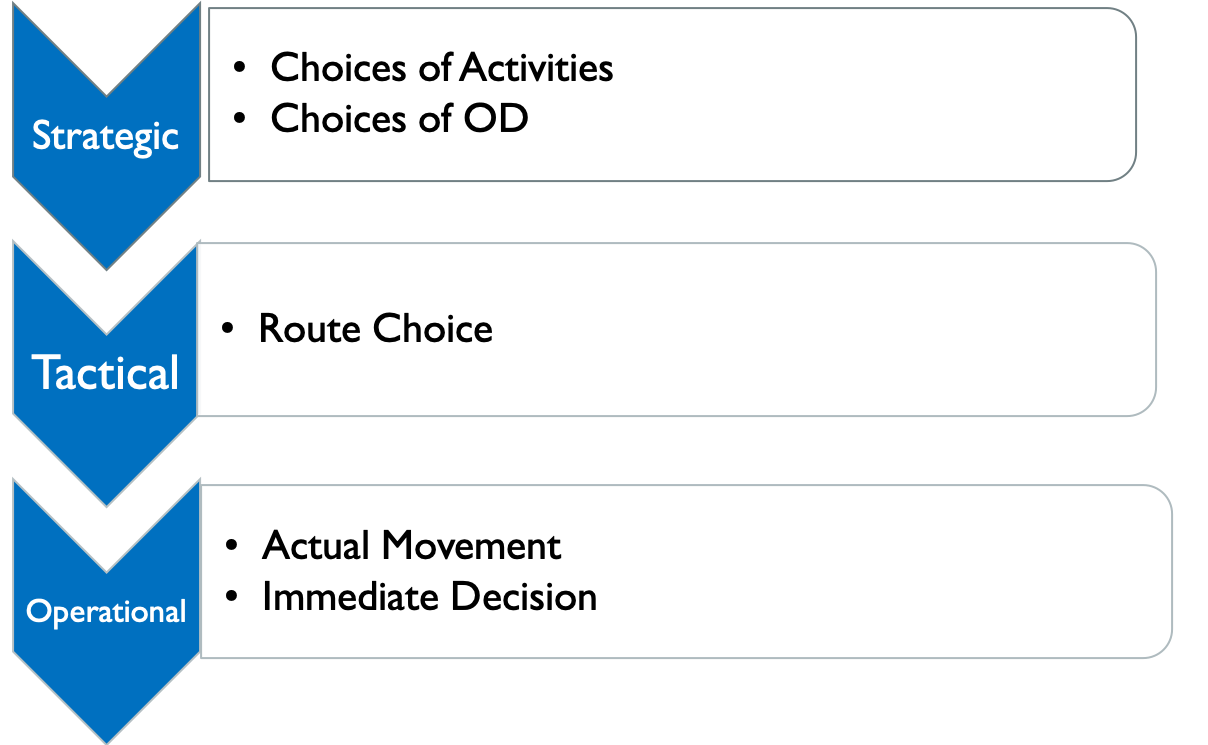
\includegraphics[scale=0.6]{chapter_1b/figures/ped-levels.png}
    \caption{Levels of behaviours for pedestrian movement modeling}
    \label{fig:model levels}
\end{figure}
In general, traditional pedestrian trajectory and movement models can be divided into two main groups: 1) Macroscopic models and 2) Microscopic models. In microscopic models, pedestrians are treated as agents, and are simulated individually. The main drawback of these type of models is the necessity of large and accurate data being available, as individual pedestrian movements require detailed information, based on different parameters. On the other side, macroscopic models consider pedestrians only in groups~\cite{sahaleh2012scenario}. The output for this type of models will then be analyzed based on fundamental diagrams. A diagram of the models discussed in this section can be observed in \cref{fig:tradtypes}, With the dark blue circles representing microscopic models, and macroscopic models represented by light blue filled circles.
\begin{figure}
    \centering
    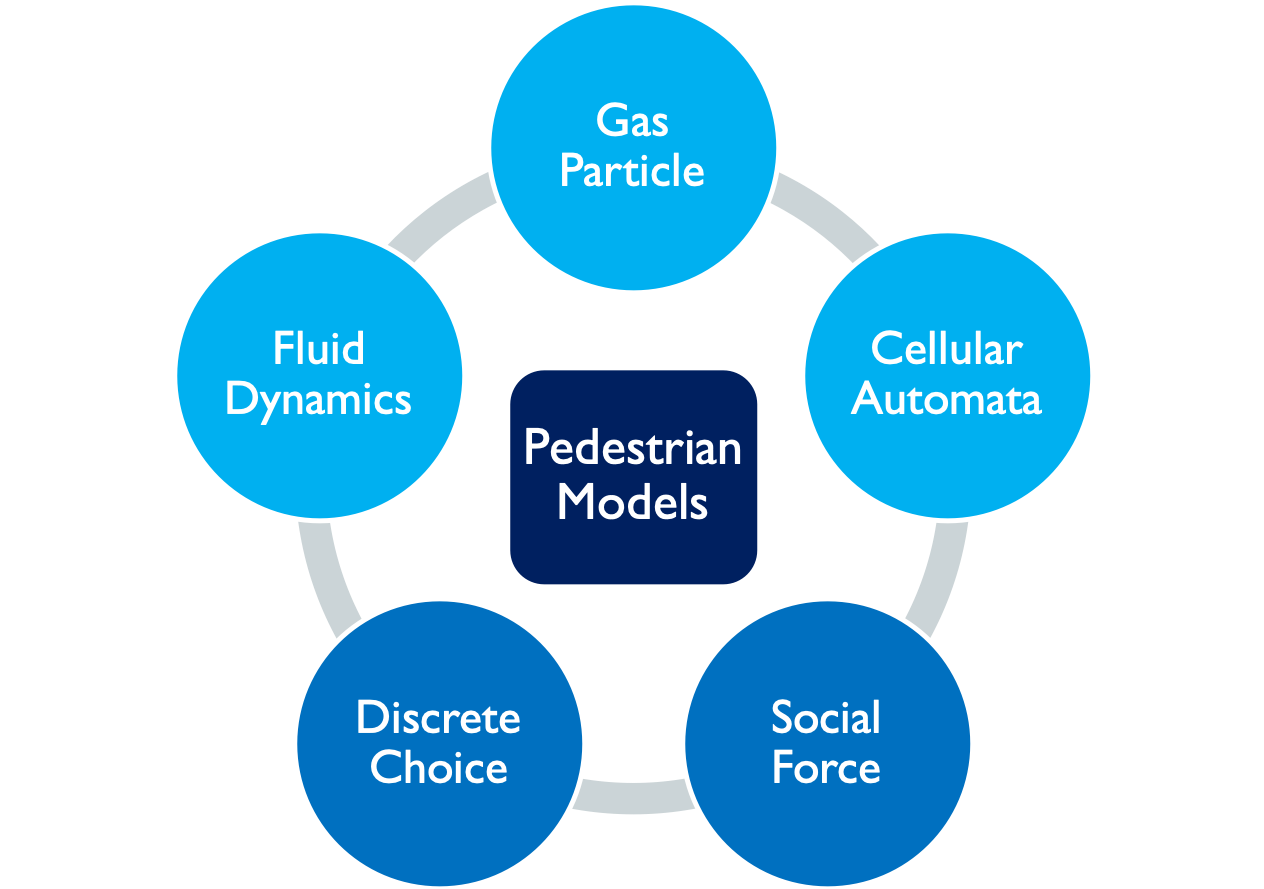
\includegraphics[scale=0.5]{chapter_1b/figures/models.png}
    \caption{Traditional pedestrian trajectory models}
    \label{fig:tradtypes}
\end{figure}
\subsubsection{Gas Particle Models}
Introduced by Henderson in 1974~\cite{henderson1974fluid}, gas particle model assumes movements of pedestrians similar to that of ideal gases. The validation of this model was done by observing data from homogeneous groups of pedestrians, i.e. pedestrians with similar gender, age, walking purpose, etc. that resemble ideal gases. In addition, such models are limited to cases where the density is high. All in all, the idea that human velocity distributions fit the Maxwell-Boltzmann distribution for the velocities of ideal gases for a given temperature, was the start of pedestrian movement modeling, and works properly if the necessary conditions are met.

\subsubsection{Fluid Dynamic Models}
Helbing~\cite{helbing1998fluid} later added some modifications to Gas particle models to account for some microscopic pedestrian phenomena, i.e. interactions between pedestrians, desire to reach a certain density, direction, exit and entrance to the system, and pedestrians reaction times. By adding the above mentioned items, a major step was taken in simulating pedestrian behaviour. Lanes of opposing flows, pedestrian jams and collisions can be observed in visualization of such models. However, low performance of the model in less congested conditions remained a problem.

\subsubsection{Cellular Automata Models}
Another popular macroscopic models for pedestrian movement modeling are cellular automated models ~\cite{blue2001cellular}. The basic concept behind this type of model is to divide the area under study into zones, called cells, and by defining some rules, pedestrians decide their movements between these zones. The first models in this category were defined by simple rules, started from Blue and Adler in 2001~\cite{blue2001cellular}, however later model incorporated more advanced probabilities for moving between cells~\cite{yamamoto2007simulation,weifeng2003simulation}.	
To apply a cellular automated model: The corridor first needs to be divided into similar square cells, with the area  \(\Delta L^2\). In each cell, pedestrians will be homogeneously distributed. To determine the route that the pedestrians choose, possible sequence of areas(contiguous sets of cells) are selected. By grouping pedestrians based on their departure times, size, route, total population in a cell is calculated as the total population of different groups within that cell in each time interval. The flow in each cell can then be calculated as: 
\begin{equation}
    \Delta Q=M.F(M/A)
\end{equation}
 in which $M$ is the population of the cell in the time interval understudy, $A$ is the area of the cell, and $F$ represents the speed-density relationship. 
 
\subsubsection{Discrete Choice Models}
In 2004, Antoninit started applying discrete choice models to pedestrian movement analysis using video recorded data~\cite{antonini2004simulation}. The microscopic approach of the model allowed detailed analysis of movements of people. The choices that the pedestrians are facing at each time in Antoninit's model are speed and direction. Utility functions for each of these choices were defined based on attributes such as presence of obstacles, proximity to the destination and positions and speed of other pedestrians. Later works on these models added other variables, helping the model gain strength by the availability of observing various factors. For instance, Guo \textit{et al.}~\cite{guo2012route} added visibility parameters to the model and Asano \textit{et al.}~\cite{asano2010microscopic} later incorporated density. The major drawback of logit-based microscopic methods is 1. their myopic nature, as they only predict the next step of a pedestrian movement without considering the big picture in terms of steps before and upcoming obstacles and 2. their requirement to discretize the space and speed into arbitrary levels.

\subsubsection{Social Force Models}
Social force model for pedestrians’ dynamics was first introduced by Helbing and Molnar in 1995~\cite{helbing1995social}, based on Lewin’s idea~\cite{lewin1951field} that behavioural changes are caused by so-called social fields. Implementing the idea on pedestrians, Helbing and Molnar described forces affecting pedestrians’ behaviours as a result of internal motivations of an individual to decide and perform actions. They categorized forces on pedestrians in three essential groups:
\begin{itemize}
    \item Forces created by acceleration to reach a desired speed,
    \item Forces that make pedestrians keep a distance to other pedestrians and objects
    \item Forces that represent attractive elements on a pedestrian walk
\end{itemize}

\subsubsection{Machine learning models for pedestrian trajectory}
Widespread success of machine learning methods in recent years, as well as the availability of large pedestrian datasets, have resulted in a shift of research trends to data-driven approaches in pedestrian studies. In one of the major earlier studies in the field, Alahi~\textit{et al.} introduced Social LSTM~\cite{alahi2016social}, a method that incorporated interactions among pedestrians in sequential models, namely Long Short-Term Memory (LSTM), to forecast trajectory of pedestrians using video footage of walking individuals in crowded scenes. In spite of the success of social LSTM model in forecasting pedestrian's trajectory, this model does not account for the contextual information on the environment and aspects like where the pedestrian is looking, thus making it difficult to apply to situations like road crossing behaviours of pedestrians in an automated environment. Furthermore, the future trajectory predicted by Social LSTM assumes a fixed length future trajectory. Lee~\textit{et al.} added semantic context to their proposed RNN model, \textit{DESIRE}~\cite{lee2017desire}, and predicted pedestrian trajectory of variable lengths in video data. More recently, Alahi~\textit{et al.} introduced \textit{Social GANs}~\cite{gupta2018social}, a model that predicts socially acceptable trajectories by training adversarial against a recurrent discriminator. 

\section{Summary}
A new approach to research on pedestrian behaviour requires modern tools on different dimensions. With the availability of big data and powerful methodological frameworks, problems of modern and future urban areas needs to be carefully defined and addressed.  In the era of big data, machine learning and neural networks are becoming an important aspect of understanding and predicting the effects of disruptive mobility on urban roads, as they offer more flexibility and computational efficiencies in handling complex data structures.

The main hypothesis of this dissertation is that by incorporating new data sources and developing novel data-driven models, communities can anticipate, and be well-aware of the changes that have started to happen in urban areas. By taking a pedestrian-oriented point of view, this dissertation seeks to provide policies and recommendations to prepare the cities for these changes, and help the dynamics of urban areas grow in a pedestrian-friendly way. 
This chapter outlined the background theory and existing research in the context of this thesis.
In the next two chapters, passively collected Wi-Fi data and Virtual Reality data are introduced and analyzed as alternative sources of data to track and count, understand and model pedestrian behaviour. \cref{chap4} and \cref{chap6} then use virtual reality data to understand pedestrian crossing behaviour in a futuristic context and in the presence of automated vehicles. Advance neural network modeling frameworks are proposed in these two chapters to replace and improve traditional models. The \textit{black box} nature of neural networks are one of the major obstacles towards a full transition to data-driven machine learning models in transportation research. To account for this concern, machine learning interpretability models are widely discussed and incorporated in this dissertation.

